\documentclass{article}
% Choose a conveniently small page size
\usepackage[paperheight=16cm,paperwidth=12cm,textwidth=10cm]{geometry}
\usepackage[utf8]{inputenc}
\usepackage[T1]{fontenc}
\usepackage{graphicx}
\usepackage{url}
\usepackage[hidelinks,breaklinks]{hyperref}
\usepackage[slovak]{babel} % vypnite pre prace v anglictine
\linespread{1.25} % hodnota 1.25 by mala zodpovedat 1.5 riadkovaniu

\title{Príklady v aplikácii Desmos}
\author{Jana Tutková}

%\usepackage{fancyhdr}
\usepackage{amsmath}
\usepackage{float}
\usepackage{amsthm}
\usepackage{amsfonts}
\usepackage{xfrac}
\usepackage{caption}
\usepackage{subcaption}
\usepackage{gensymb}
\usepackage{mathtools} 

\usepackage{pgfplots}
\pgfplotsset{compat=1.18, width=10cm}

\usepackage{multirow}
\usepackage{adjustbox}
\newcommand{\altref}[2]{\hyperref[#1]{#2}}

\usepackage[labelformat=simple]{subcaption}
\renewcommand\thesubfigure{(\alph{subfigure})}

\begin{document}
\maketitle
\begin{figure}[h]
	\centering
    \captionsetup{justification=centering}
	\captionsetup[subfigure]{justification=centering}
	\begin{subfigure}[t]{0.49\textwidth}
		\centering
		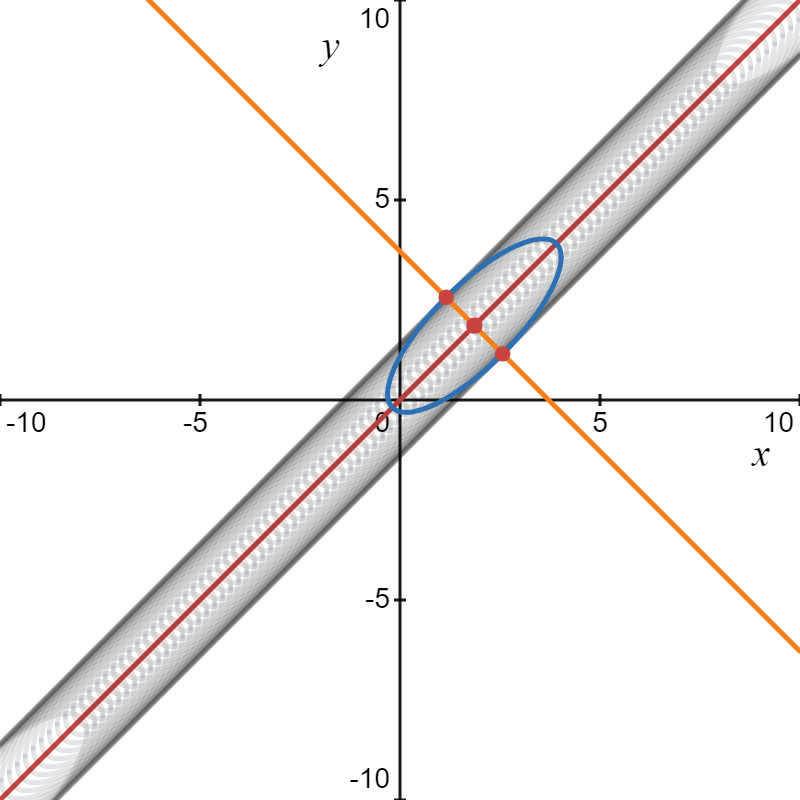
\includegraphics[width=0.5\textwidth]{images/line_desmos.png}
		\caption{Priamka $m(t)=(ct, dt).$ \\
		\url{https://www.desmos.com/calculator/3zjk617ien}.}
		\label{fig:priamka}
	\end{subfigure}
    \hfill
    \begin{subfigure}[t]{0.49\textwidth}
        \centering
		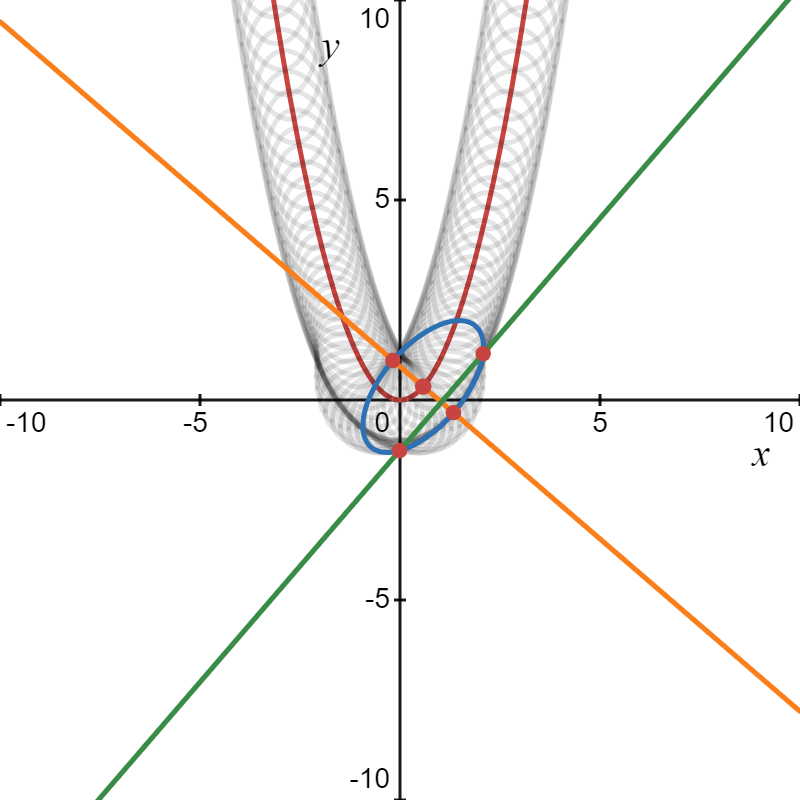
\includegraphics[width=0.5\textwidth]{images/parabola_desmos.png}
		\caption{Parabola $m(t)=(t, t^2).$ \\
		\url{https://www.desmos.com/calculator/bmcg8btqml}.}
		\label{fig:parabola}
	\end{subfigure}
    \hfill
    \begin{subfigure}[t]{0.49\textwidth}
        \centering
		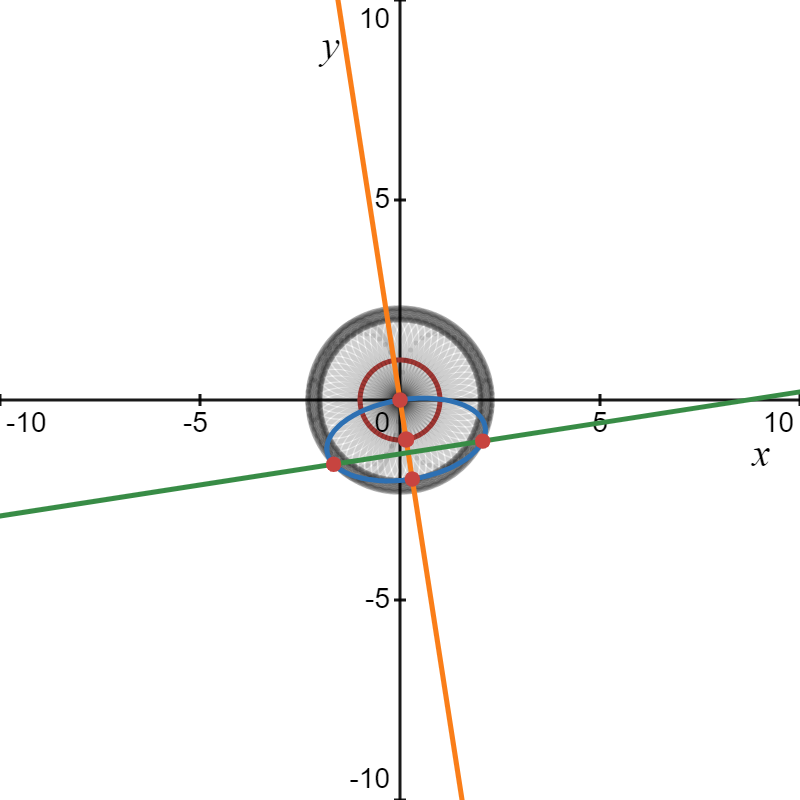
\includegraphics[width=0.5\textwidth]{images/kruznica_desmos.png}
		\caption{Kružnica $m(t)=(\cos t, \sin t).$ \\
		\url{https://www.desmos.com/calculator/fmqyd42xcc}.}
		\label{fig:kruznica}
	\end{subfigure}
    \hfill
    \begin{subfigure}[t]{0.49\textwidth}
        \centering
		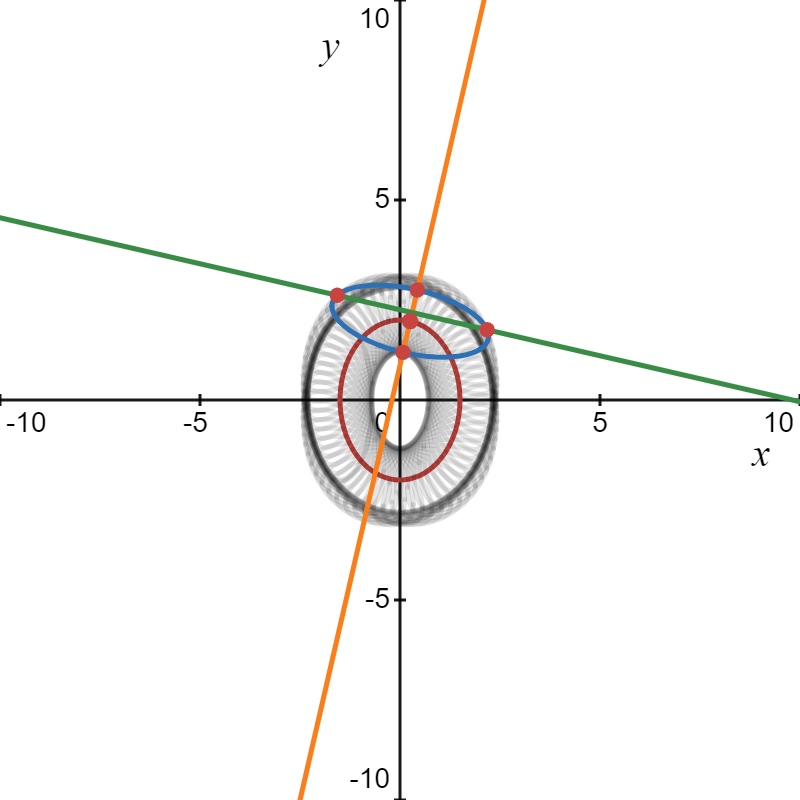
\includegraphics[width=0.5\textwidth]{images/elipsa_desmos.png}
		\caption{Elipsa $m(t)=(c \cos t, d \sin t).$ \\
		\url{https://www.desmos.com/calculator/ujuow2jlnr}.}
		\label{fig:elipsa}
	\end{subfigure}
    \hfill
    \begin{subfigure}[t]{0.49\textwidth}
        \centering
		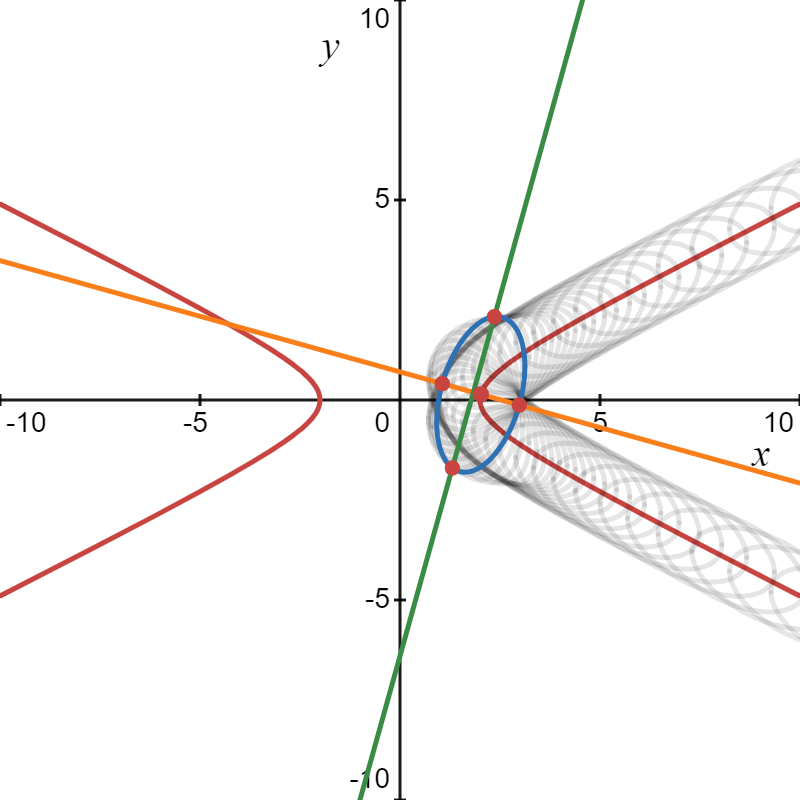
\includegraphics[width=0.5\textwidth]{images/hyperbola_desmos.png}
		\caption{Hyperbola $m(t)=(c \cosh t, d \sinh t).$ \\
		\url{https://www.desmos.com/calculator/zhu3u0nucj}.}
		\label{fig:hyperbola}
	\end{subfigure}
%    \hfill
%    \begin{subfigure}[t]{0.49\textwidth}
%        \centering
%		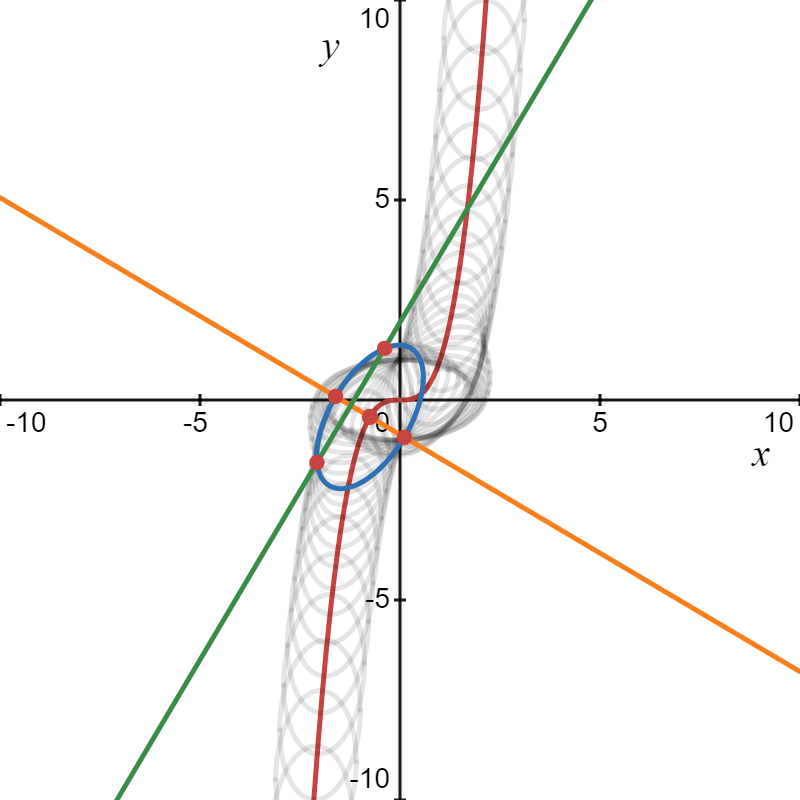
\includegraphics[width=0.5\textwidth]{images/kubicka_desmos.png}
%		\caption{Kubická krivka $m(t)= (t, t^3).$ \\
%		\url{https://www.desmos.com/calculator/cophsjqq8j}.}
%		\label{fig:kubicka}
%	\end{subfigure}
    \hfill
    \begin{subfigure}[t]{0.49\textwidth}
        \centering
		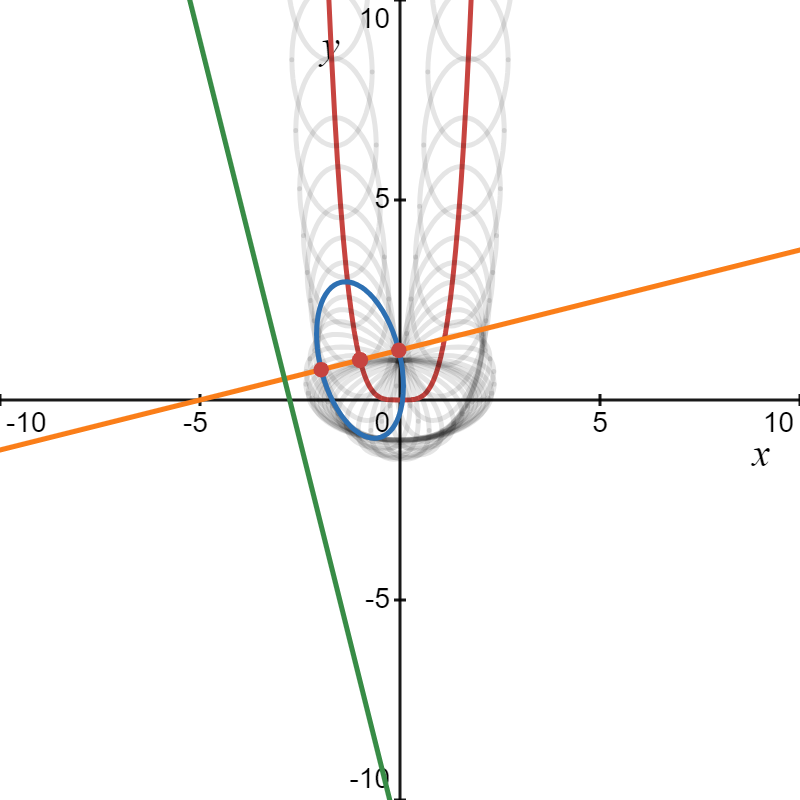
\includegraphics[width=0.5\textwidth]{images/kvarticka_desmos.png}
		\caption{Kvartická krivka $m(t)= (t, t^3).$\\
		\url{https://www.desmos.com/calculator/bcqreazezc}.}
		\label{fig:kvarticka}
		\end{subfigure}
\end{figure}
\end{document}